\documentclass[a4paper]{article}

\usepackage{color}
\usepackage{url}
\usepackage[utf8]{inputenc}
%\usepackage[T1]{fontenc}
\usepackage{graphicx}
\usepackage{listings}
%\usepackage{matlab-prettifier}
%\usepackage{comment}

\usepackage{amsmath}
\usepackage{color}
\usepackage{url}
\usepackage{hyperref}


%\def\d{{\fontencoding{T1}\selectfont\dj}}
%\def\D{{\fontencoding{T1}\selectfont\DJ}}

\def\dj{d\kern-0.4em\char"16\kern-0.1em}
\def\Dj{\mbox{\raise0.3ex\hbox{-}\kern-0.4em D}}
%\newcommand\D{D\kern-0.8em\raise0.2ex\hbox{--}\kern0.3em}

%\usepackage[utf8]{hyperref}
\hypersetup{colorlinks,citecolor=green,filecolor=green,linkcolor=blue,urlcolor=blue}


\renewcommand{\contentsname}{Sadržaj}
\renewcommand{\abstractname}{Sažetak}
\renewcommand{\figurename}{Slika}
\renewcommand{\refname}{Literatura}

\begin{document}
	\title{Kitovi \\ \small{Seminarski rad u okviru kursa\\Osnovi matematičkog modeliranja\\ Matematički fakultet}}
	
	\author{Nataša Blagojević \\ mi20159@alas.mat.bg.ac.rs \and Lazar Lazović \\ mi20062@alas.matf.bg.ac.rs}
	\date{28.~maj 2024.}
	\maketitle
	
	\abstract{U ovom radu ćemo se upoznati sa dinamikom populacije plavih kitova i kitova perajara koristeći matematički model. Analiziramo stacionarne tačke sistema, numerički rešavamo model, istražujemo uticaj promene prirodnog priraštaja plavih kitova i uključujemo ribarenje kako bismo odredili optimalni broj brodova radi održavanja ravnoteže u populaciji kitova.
		
	\tableofcontents
		
	\newpage
		
	
	\section{Uvod}
	%\label{sec: Uvod}
	
	Pupulacija morskih sisara ima ključnu ulogu u održavanju ravnoteže u morskim ekosistemima. Plavi kitovi i kitovi perajari su značajni predstavnici ovih populacija, čija dinamika može biti složena i podložna različitim uticajima okoline. Međutim, aktivnost kao što je ribolov može imati značajan uticaj na ove populacije, što zahteva pažljivo istraživanje i analizu. \\
	\\
	U ovom radu istražujemo kako se dinamika populacije plavih kitova i kitova perijara menja kroz matematički model koji uzima u obzir faktore kao što su dostupnost hrane(planktona), međusobno nadmetanje, prirodni priraštaj i uticaj ribolova. Modeliranje ovakvih složenih sistema nam omogućava bolje razumevanje i ponašanje sisara pod različitim uslovima, kao i pružanje smernica za upravljanje i očuvanje ovih vrsta u prirodi.  \\ 
	\\
	Naša analiza se oslanja na sistem diferencijalnih jednačina koje opisuju promene u populacijama plavih kitova (\textit{x(t)}) i kitova perajara (\textit{y(t)}) u odnosu na vreme \textit{t}. Model uzima u obzir reprodukciju populacije, međusobno nadmetanje za hranu i prirodni priraštaj definisanih pomoću parametara koji karakteristišu ove procese. \\
	\\
	Cilj našeg istraživanja je da istražimo kako međusobno nadmetanje, prirodni priraštaj i ribolov utiče na samu dinamiku populacija plavih kitova i kitova perajara, kao i kako se ove promene odražavaju na stabilnost i dugoročno održavanje ovih populacija. \\ 
	\\ 
	U nastavku ovog rada, predstavljamo detaljnu analizu našeg matematičkog modela, rezultate simulacija za različite scenarije, kao i diskusiju o analizama za očuvanje ovih morskih sisara.
	
	\section{Matematički model}
	\label{sec: matematocki-model}
	
	Predstavljamo matematički model koji opisuje dinamiku promene populacije jedinki plavih kitova i kitova perajara koji se takmiče za hranu (planktone). \\
	\\
	Neka su \textit{x(t)} i \textit{y(t)} označeni kao ukupan broj plavih kitova i kitova perajara u trenutku \textit{t}. Parametar \textit{a} je pozitivan parametar koji predstavlja intezitet konkurencije između ove dve vrste za zajedničke resurse, a to je hrana. \\ 
	\\ 
	Sistem diferencijalnih jednačina koji opisuje dinamiku populacije je dat sa: \\
	
	\[
		\frac{dx}{dt} = 0.05x(1 - \frac{x}{250000}) - axy
 	\] 
 	
 	\[
 		\frac{dy}{dt} = 0.08y(1 - \frac{y}{400000}) - axy 
 	\] 
 	\\
 	
 	Prva jednačina opisuje kako se broj plavih kitova menja tokom vremena. Prvi član, tj. $0.05x(1 - \frac{x}{250000})$ predstavlja  prirodni priraštaj broja plavih kitova, gde se brzina rasta smanjuje kako populacija plavih kitova približava kapacitetu staništa od 250000. Drugi član, tj. $-axy$ opisuje negativan uticaj konkurencije između plavih kitova i kitova perajara na rast populacije plavih kitova.\\ 
 	\\	
	Promena broja kitova perajara u odnosu na vreme opisana je drugom jednačinom. Prvi član na desnoj strani, tj. $0.08y(1 - \frac{y}{400000})$ predstavlja prirodni poriraštaj kitova perajara, gde se stopa rasta takođe smanjuje s povećanjem broja kitova perajara, ali opada kako se populacija približava kapacitetu staništa od 400000. Drugi član,tj. $-axy$ predstavlja negativan uticaj konkurencije između plavih kitova i kitova perajara na rast populacije kitova perajara.\\
	\\
	Početni uslovi ovog modela su da na početku imamo 6000 jedinki plavog kita i 60000 jedinki kitova perajara.  
	
	
	\section{Stacionarana rešenja}
	\label{sec: stacionarna-resenja}
	
	Za pronalaženje stacionarnih rešenja modela koji opisuje dinamiku plavih kitova i kitova perajara, koristimo metod stavljanja diferencijalnih jednačina u stanje ravnoteže, gde se brzine promena populacije izjednačavaju sa nulom. \\ 
	\\ 
	Model je definisan na sledeći način:
	
	\begin{equation}
		\frac{dx}{dt} = 0.05x(1 - \frac{x}{250000}) - axy
	\end{equation}
	
	\begin{equation}
		\frac{dy}{dt} = 0.08y(1 - \frac{y}{400000}) - axy
	\end{equation}
	\\
	Gde nam \textit{x} i \textit{y} predstavljaju populacije plavih kitova i kitova perajara, dok je \textit{a} parametar koji nam opisuje uticaj međusobnog nadmetanja.\\
	\\
	Kako bismo pronašli stacionarna rešenja, potrebno je da obe jednačine izjednačimo sa nulom, jer nam stacionarna rešenja predstavljaju ona rešenja u kojima se populacija kitova ne menja tokom vremena.\\
	
	\newpage
	
	Za zadati parametar $a = 10^{-8} $ i za zadate početne uslove da je na početku 6000 jedinki plavog kita i 60000 jedinki kita perajara. Rešavamo početni sistem na malopređašnji opisani način. \\ 
	\\

	Precizna definicija početnih uslova (*): \\
	\[
		a = 10^{-8}
	\]
	\[
		x(0) = 6000
	\]

	\[
		y(0) = 60 000
	\]
	
	Izjednačavanje obe jednačine sa 0:
	
	\begin{equation}
		\frac{dx}{dt} = 0 
	\end{equation}

	\begin{equation}
		\frac{dy}{dt} = 0
	\end{equation}
	
	Dobijamo sledeće sisteme:
	
	\begin{equation}
		0.05x(1 - \frac{x}{250000}) - axy = 0
	\end{equation}
	
	\begin{equation}
		0.08y(1 - \frac{y}{400000}) - axy = 0
	\end{equation}
		
	Potom dobijamo:
	
	\[
		x(0.05(1 - \frac{x}{250000}) - ay) = 0
	\]
	
	\[
		y(0.08(1 - \frac{y}{400000}) - ax) = 0
	\]
	
	Odnosno: 
	
	\begin{equation}
		x = 0   \vee    0.05 \cdot (1 - \frac{x}{250000}) - ay = 0
	\end{equation}

	\begin{equation}
		y = 0   \vee    0.08 \cdot (1 - \frac{y}{400000}) - ax = 0
	\end{equation}
		
	Rešavanjem ovako dobijenog sistema, odmah mozemo uočiti trivijalno rešenje, a to je par $(x, y) = (0, 0)$. \\
	\\
	Kako znamo da nam je $x = 0$, tu vrednost možemo uvrstiti u izraz $0.08 \cdot (1 - \frac{y}{400000}) - ax = 0$, pri čemu znamo da je $a = 10^{-8}$. Sređivanjem ovog izraza dobijamo da je $y = 400000$. \\
	Tako ubacujemo i vrednost $y = 0$ u izraz $0.05 \cdot (1 - \frac{x}{250000}) - ay = 0$. Znamo da nam je $a = 10^{-8}$ i kada sve sredimo, dobijamo $x = 250000$. \\
	\\
	Ovim računanjem smo dobili još dva para rešenja, a to su: $(x, y) = (0, 400000)$ i $(x, y) = (250000, 0)$.\\
	\\
	Rešavanjem sledećeg sistema, dobijamo još jedan par koji predstavlja stacionarno rešenje.\\
	\\	  
	
	%Jedno stacionarno rešenje nam predstavlja par $(x, y) = (0, 0)$, a nas zanima drugo stacionarno rešenje koje se dobija rešavanjem sistema:
	\newpage
	
	\[
		0.05 \cdot (1 - \frac{x}{250000}) - ay = 0
	\]
	
	i 
	
	\[
		0.08 \cdot (1 - \frac{y}{400000}) - ax = 0
	\]
	
	Zamenjujemo parametar a sa vrednošću: $a = 10^{-8}$ i dobijamo sledeće jednačine:
	
	\begin{equation}
		0.05 \cdot (1 - \frac{x}{250000}) - 10^{-8} y = 0
	\end{equation}

	\begin{equation}
		0.08 \cdot (1 - \frac{y}{400000}) - 10^{-8} x = 0
	\end{equation}

	%\newpage

	Iz jednačine (7) izrazimo y:
	
	\[
		y = 10^8 \cdot 0.05 \cdot (1 - \frac{x}{250000})
	\]

	Kada malo bolje raspišemo i sredimo izraz za \textit{y} dobijamo sledeću jednačinu: 
	
	\begin{equation}
		y = 5 \cdot 10^6 - 20x
	\end{equation}

	Potom izraženo y iz jednačine (11) uvrstimo u jednačinu (10) i dobijamo sledeće: 
	
	\[
		0.08 \cdot (1 - \frac{5 \cdot 10^6 - 20x}{400000}) - 10^{-8} x = 0  
	\]
	
	Nakon detaljnijeg matematičkog računa dobijamo sledeću jednakost:
	
	\begin{equation}
		399x = 92 \cdot 10^6
	\end{equation} 

	Odatle dobijamo da je $ x \approx 230576 $. Kada ovo rešenje uvrstimo u jednačinu (11) dobijamo približnu vrednost za y, a to je $ y \approx 388480 $.  
	
	\subsection{Analiza stacionarnih rešenja}
	\label{sec: analia-stacionarnih-resenja}
	
	Kao jedno stacionarno rešenje dobili smo par $ (x, y) = (0, 0)$. Ovo rešenje znači da nijedna populacija nema prisustva u ekosistemu. To može ukazivati na izumiranje obe vrste kitova ili na nepovoljne uslove sredine koje ne podržavaju njihov opstanak. Ovo stacionarno rešenje je trivijalno i stoga ne predstavlja realističan scenarijo za ekološki sistem.\\
	\\
	Drugo stacionarno rešenje koje smo dobili je $ x \approx 230576$ i $ y \approx 388480$. Ovo rešenje predstavlja situaciju u kojoj su populacije plavih kitova i kitova perajara prisutne u ekosistemu, odnosno da postoji neka određena ravnoteža između kitova.\\
	\\
	Sada proveravamo koja su to rešenja stabilna. To cemo uraditi uz pomoć MATLAB-a u kojem ćemo napisati kod koji nam računa matricu, na osnovu koje ćemo utvrditi da li je naše malopređašnje rešenje stabilno ili nestabilno.
	
	\iffalse
	%\begin{flushleft}
		\begin{lstlisting}[language=Matlab]
		function analyze_stability(stationary_point, a)
		% Izdvajanje koordinata stacionarnog resenja
		x_star = stationary_point(1);
		y_star = stationary_point(2);
		
		% Izracunavanje Zordanove matrice u stacionarnoj tacki
		J = [0.05*(1 - 2*x_star/250000) - a*y_star, -a*x_star;
		-a*y_star, 0.08*(1 - 2*y_star/400000) - a*x_star];
		
		% Procena sopstvenih vrednosti Zordanove matrice
		eigenvalues = eig(J);
		
		% Prikaz rezultata
		disp('Zordanova matrica:');
		disp(J);
		disp('Sopstvene vrednosti:');
		disp(eigenvalues);
		
		% Provera stabilnosti
		if all(real(eigenvalues) < 0)
		disp('Stacionarno resenje je stabilno.');
		else
		disp('Stacionarno resenje je nestabilno.');
		end
		end
		
		\end{lstlisting}
	%\end{flushleft}	
	\fi
	
	Funkcija \textbf{analyse\_stability} prvo izračunava Žordanovu matricu u datoj stacionarnoj tački i potom procenjuje sopstvene vrednosti i utvrđuje stabilnost rešenja. Pozivamo je na sledeći način:\\ 
	
	\[
		analyse\_stability([230576, 388480], 1e-8);
	\]
	
	
	Nakon izvršenja analize stabilnosti, dobijamo sledeću Žordanovu matricu i sopstvene vrednosti u tački stacionarnog rešenja ((230576, 388480)), za dati parametar ($a = 10^{-8}$):
	\[
		\begin{bmatrix}
			-0.0461 & -0.0023 \\
			-0.0038 & -0.0777 \\
		\end{bmatrix} 
	\]	
	
	i sledeće sopstevene vrednosti:
	
	\[
		\lambda_1 \approx -0.0458
	\]
	
	\[
		\lambda_2 \approx -0.780
	\]
	
	Oba sopstvena vektora su realna i negativna, što ukazuje na to da su obe sopstvene vrednosti negativne. Odatle zaključujemo da je stacionarno rešenje $(230576, 388480)$ stabilno. \\
	\\ 
	To znači da u dugoročnom stabilnom stanju da se populacije plavih kitova i kitova perajara održavaju na nivou koji odgovara tački stacionarnog rešenja. Sistem će se vratiti na ovo stabilno stanje nakon bilo kakvih manjih poremećaja, što ukazuje na ravnotežu između reprodukcije, smrtnosti i drugih faktora koji utiču na populaciju kitova. \\
	\\
	Sada izanalizirajmo sledeće stacionarno rešenje: $(x, y) = (250000, 0)$. Ako pokrenemo istu funkciju, samo za različite parametre x i y, dobićemo sledeću Žordanovu matricu:\\
	
	\[
		\begin{bmatrix}
			-0.05 & -0.0025 \\
			    0   & 0.0775 \\
		\end{bmatrix} 
	\]
	
	Odnosno, sledeće sopstvene vrednosti:
	
	\[
		\lambda_1 = -0.05
	\] 
	
	\[
		\lambda_2 = 0.0775
	\]
	
	Kako imamo pozitivno prisustvo parametra $\lambda_2$, to nam ukazuje da je ovo rešenje nestabilno. Nestabilnost ove tačke nam govori da teoretski populacija kitova perajara može da preživi bez plavih kitova. Iz stvarnog sveta gledano, bilo koje malo odstupanje može dovesti do promene dinamike sistema, što znači da nije verovatno da će ovakav scenarijo biti dugoročan. Gledano sa ekološke strane, populacija plavih kitova izumire, dok se populacija kitova perajara dostiže ravnotežnu tačku od 400000 jedinki. \\
	\\
	Razmotirmo još jedno stacionarno rešenje: $(x, y) = (0, 400000)$. Računamo Žordanovu matricu uz pomoć prethodne funkcije i dobijamo:
	
	
	\[
		\begin{bmatrix}
			0.046  &   0  \\
			-0.004 & -0.0800 \\
		\end{bmatrix} 
	\]	
	
	\newpage
	
	Sopstvene vrednosti za ovu matricu su:
	
	\[
		\lambda_1 = -0.08
	\]
	
	\[
		\lambda_2 = 0.046
	\]
	
	Kao i u prethodnom slučaju, pozitivna vrednost $\lambda_2$ nam sugeriše da je ovo stacionarna tačka nestabilna. Nestabilnost ove tačke nam govori da teoretski populacija plavih kitova može da preživi bez kitova perajara. U stvarnosti, bilo kakvo malo odstupanje mogu da dovedu do promene dinamike sistema, a to znači da nije verovatno da će ovakav scenarijo biti dugoročan. Iz ekološke tačke gledišta, ovo je scenarijo u kojem populacija kitova perajara izumire, dok populacija plavih kitova dostiže ravnotežnu tačku od 250000 jedinki.\\
	\\
	%Stacionaran rešenja $(x, y) = (25000, 0)$ i $(x, y) = (0, 400000)$ nam upućuju na mogućnost da konkurencija između dve vrste može dovesti do izumiranja jedne od njih. U oba scenarija, jedna vrsta izumire dok druga preživljava, što ukazije na visoku konkurenciju za zajedničke resurse
	
	Iako nam stacionarna rešenja ukazuju na moguće ravnotežne tačke gde jedna vrsta može da preživi bez druge, njihova nestabilnost govori da je ovako nešto nemoguće postići u prirodi. 
		
	\section{Numeričko rešavanje modela i grafički prikaz}
	\label{sec:nrmgp}	
	
	
	Kako bismo numerički rešili model za parametre $a = 10^{-8}$ i $a = 10^{-6}$, potrebno ih je uvrstiti u diferencijalne jednačine i potom primenom numeričkih metoda rešiti sistem diferencijalnih jednačina. Zatim ćemo grafički prikazati broj jedinki obe vrste kitova u zavisnosi od vremena i nakon toga ćemo diskutovati o ponašanju sistema kada $t \to \infty$.  
	
	\begin{figure}[h]
		\centering
		\begin{minipage}[h]{0.45\linewidth}
			\centering
			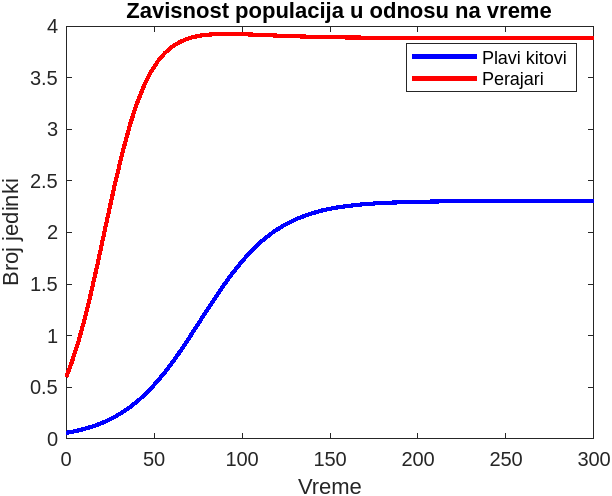
\includegraphics[width=\textwidth]{a8.png}
			\caption{$a = 10^{-8}$}
			\label{slika1:model_e8}
		\end{minipage}
		\hspace{0.5cm} 
		\begin{minipage}[h]{0.45\linewidth}
			\centering
			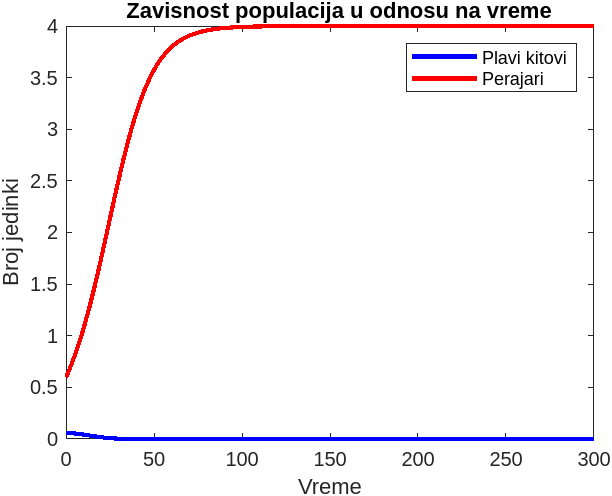
\includegraphics[width=\textwidth]{a6.png} 
			\caption{$a = 10^{-6}$} 
			\label{slika2:model_e6}
		\end{minipage}
	\end{figure}
	
	\newpage	

	Parametar \textit{a} nam predstavlja međusobno nadmetanje između vrsta, različite vrednosti rezultiraju različitim dinamikama populacije. Manja vrednost ($a = 10^{-8}$) nam ukazuje na to da će nadmetanje između vrsta biti manje, što za posledicu ima da se obe vrste populacija kitova povećava (Slika 1). A, sa druge strane za $a = 10^{-6}$ nam ukazuje na intezivnije međusobno nadmetanje, što za posledicu ima izumiranje plavih kitova (Slika 2). \\ 
	\\ 
	\subsection{Detaljna analiza za $a = 10^{-8}$}
	\label{sec: Dmodel_e8}
	
	Kako imamo manju konkurenciju za resurse, kao što su u ovom slučaju hrana, omogućava svakoj populaciji veći pristup neophodnim resursima za opstanak. Očekujemo da će konkurencija među populacijama biti manje izražena, populacije će imati veću tendeciju da dostignu stabilne tačke u kojima nema značajnih promena tokom vremena ili će te promene biti sporije. Tako da, kada nam vreme teži beskonačnosti, odnosno $t \to \infty$, populacije će težiti svojim stabilnim tačkama.
			
	\subsection{Detaljna analiza za $a = 10^{-6}$}
	\label{sec: Dmodel_e6}
	
	Očekujemo da će nadmetanje između plavih kitova i kitova perajara biti više izražena. Održava intezitet konkurencije između ove dve vrste za zajedničke resurse. Kako je parametar za nadmetanje veći, to će imati veći uticaj na promenu populacije. Kada analiziramo samu dinamiku sistema, očekujemo da će populacija kitova perajara dostići stabilnu tačku, gde će se broj jedinki stabilizovati na određenom nivou. Zbog intezivnije konkurencije i većeg uticaja parametra nadmetanja, populacija plavih kitova će izumreti. 
		
	
	\section{Prirodni priraštaj}
	\label{sec: prirodni-prirastaj}
	
	Prirodni priraštaj predstavlja ključni faktor u dinamici populacija u prirodi. Njegova uloga u održavanju stabilnosti ekosistema i dugoročnog opstanka vrsta je od suštinskog značaja. \\
	\\
	Prirodni priraštaj jedna je od osnovnih komponenti koja utiče na promene u populaciji plavih kitova. Ona se definiše kao stopa kojom se populacija povećava ili smanjuje zbog prirodnih procesa kao što su reprodukcija, smrtnost, migracija i slično. \\ 
	\\
	Sledeća jednačina predstavlja matematički model koji u odnosu na prethodni uključuje i prirodni priraštaj (u jednačini označen sa \textit{p}) u razmatranje: \\ 
	\[
		\frac{dx}{dt} = px \cdot (1 - \frac{x}{250000}) - axy
	\]
	
	Izanaliziraćemo konkretne slučajeve za prirodni priraštaj i njegov uticaj na dinamiku populacije plavih kitova. Fiksiraćemo $a = 10^{-8}$ za parametar razmatraćemo vrednosti 2\%, 3\%, 4\%, 6\%, 7\%. \\
	
	\iffalse
	
	\begin{figure}[h]
		\centering
		\begin{minipage}[h]{0.45\linewidth}
			\centering
			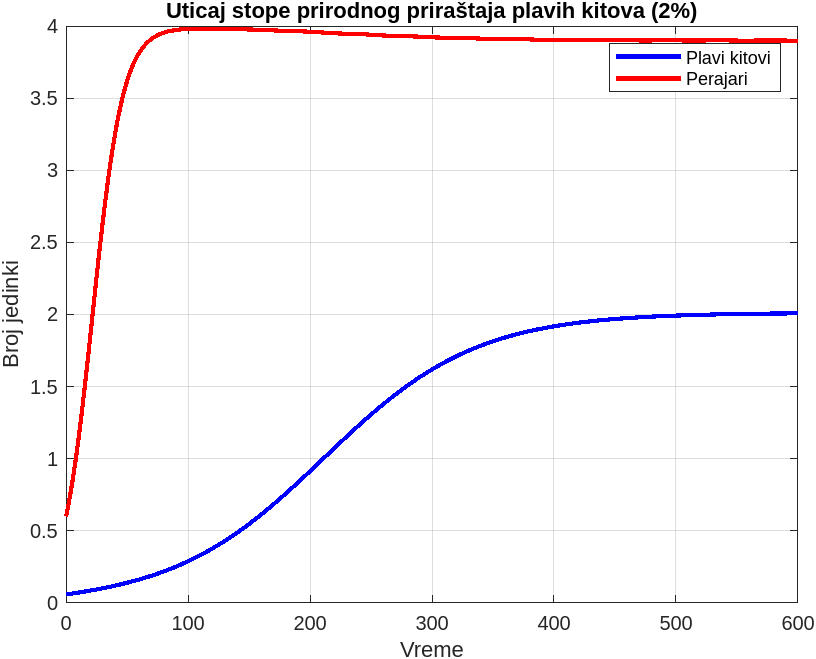
\includegraphics[width=\textwidth]{uticaj2.png}
			\caption{Priraštaj za 2\%}
			\label{slika1: pp2}
		\end{minipage}
		\hspace{0.5cm} 
		\begin{minipage}[h]{0.45\linewidth}
			\centering
			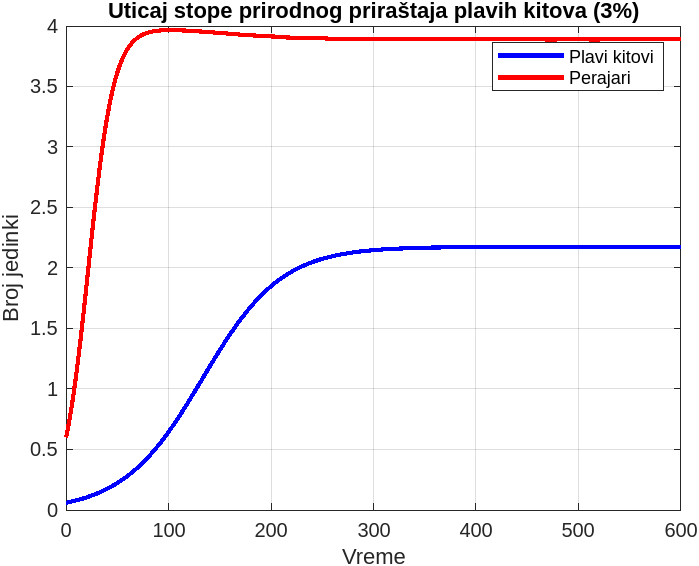
\includegraphics[width=\textwidth]{uticaj3.png} 
			\caption{Priraštaj za 3\%} 
			\label{slika2: pp3}
		\end{minipage}
	\end{figure}

	\begin{figure}[h]
		\centering
		\begin{minipage}[h]{0.45\linewidth}
			\centering
			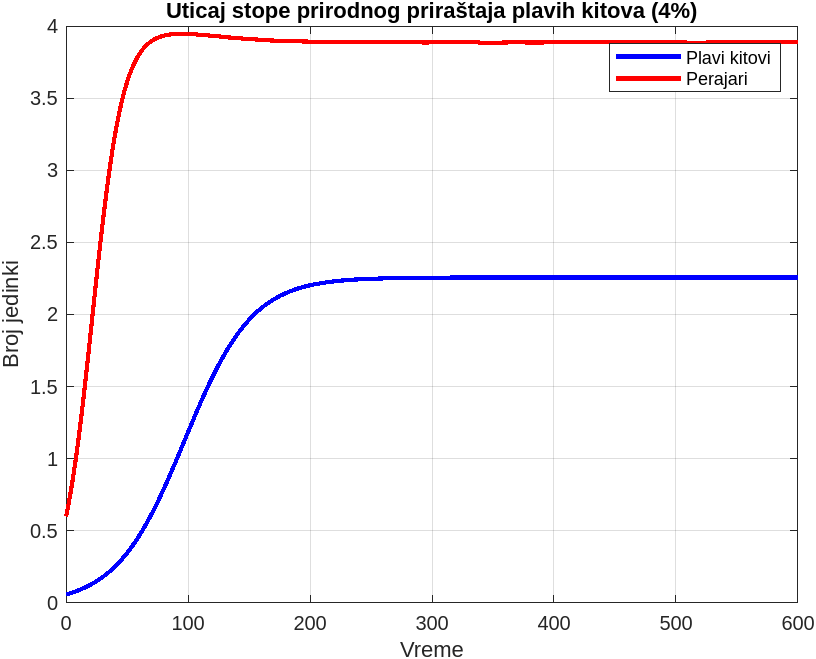
\includegraphics[width=\textwidth]{uticaj4.png}
			\caption{Priraštaj za 4\%}
			\label{slika1: pp4}
		\end{minipage}
		\hspace{0.5cm} 
		\begin{minipage}[h]{0.45\linewidth}
			\centering
			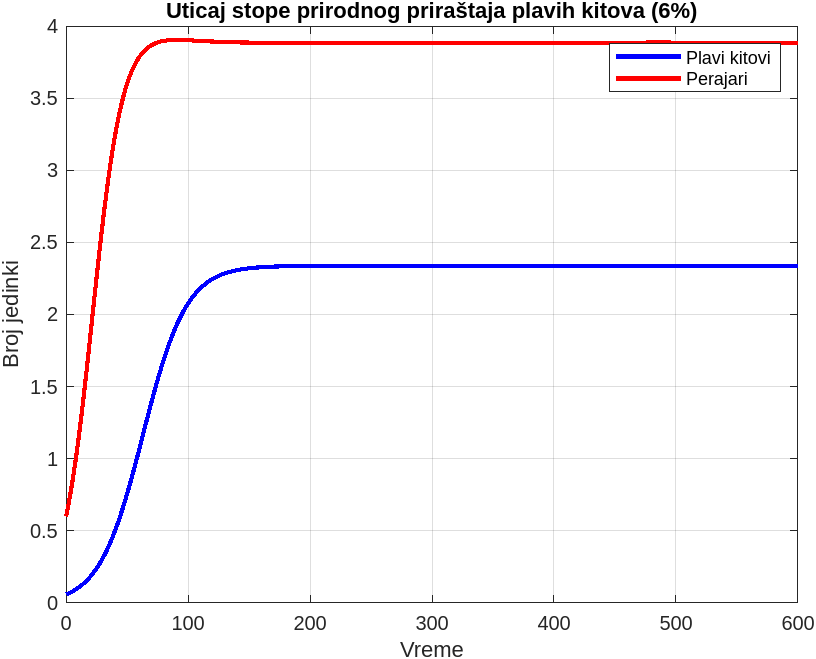
\includegraphics[width=\textwidth]{uticaj6.png} 
			\caption{Priraštaj za 6\%} 
			\label{slika2: pp6}
		\end{minipage}
	\end{figure}

	\begin{figure}[h]
		\centering
		\begin{minipage}[h]{0.45\linewidth}
			\centering
			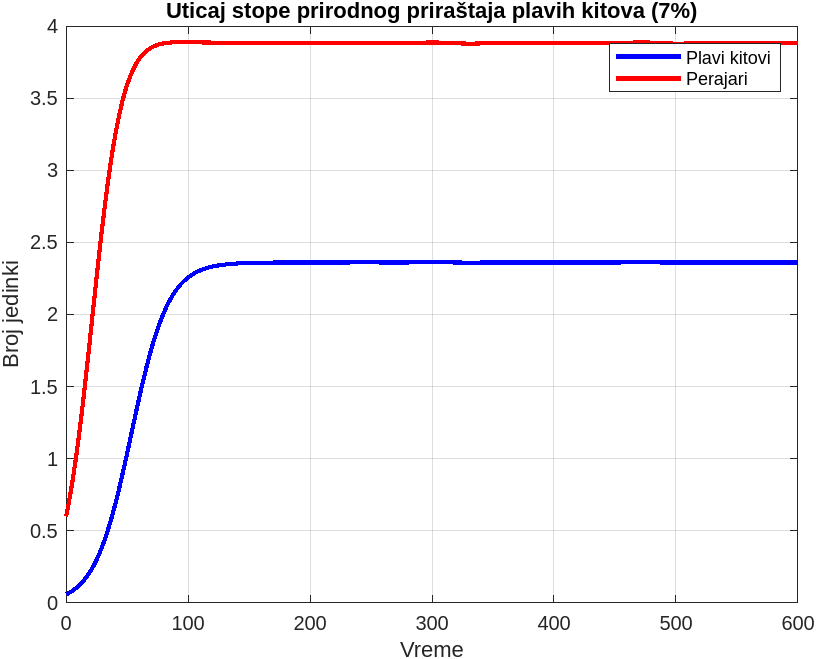
\includegraphics[width=\textwidth]{uticaj7.png}
			\caption{Priraštaj za 7\%}
			\label{slika1: pp7}
		\end{minipage}
	\end{figure}
	
	\newpage
	
	Zaključujemo da povećanjem parametra prirodnog priraštaja populacija raste brže nego pre, odnosno plavi kitovi će brže nego pre dostići stabilnu tačku.
	
	\fi 
	
	\newpage
	
	\subsection{Niska stopa priraštaja (2\%)}
	\label{sec: niska-stopa-prirastaja}
	
	\begin{figure}[h]
		\centering
		\begin{minipage}[h]{0.45\linewidth}
			\centering
			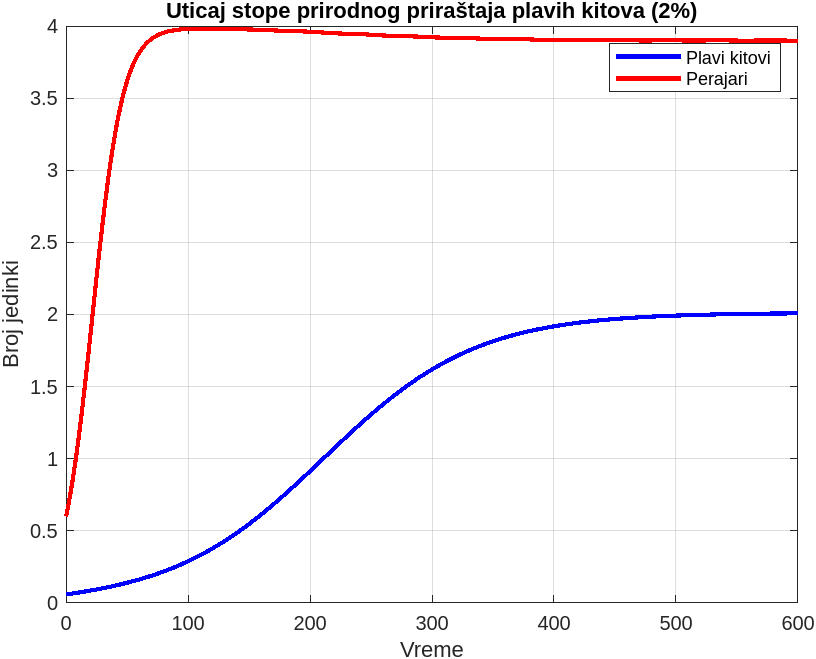
\includegraphics[width=\textwidth]{uticaj2.png}
			\caption{Priraštaj za 2\%}
			\label{slika1: uticaj2}
		\end{minipage}
	\end{figure}

	Sa prirodnim priraštajem od 2\%, sa grafika (Slika 3) uočavamo spor rast populacije plavih kitova. Početna populacija će polako da raste, a efekti sa konkurencijom kitova perajara će imati manji uticaj na početku zbog nižeg rasta broja jedinki. Populacija plavih kitova će dostići stabilnu tačku, ali im je za to potrebno dosta vremena. Stacionarna tačka će biti niska u poređenju sa višim stopama prirodnog priraštaja.
	
	
	\subsection{Umerena stopa priraštaja (3-4\%)}
	\label{sec: umerena-stopa-prirastaja}
	
	\begin{figure}[h]
		\centering
		\begin{minipage}[h]{0.45\linewidth}
			\centering
			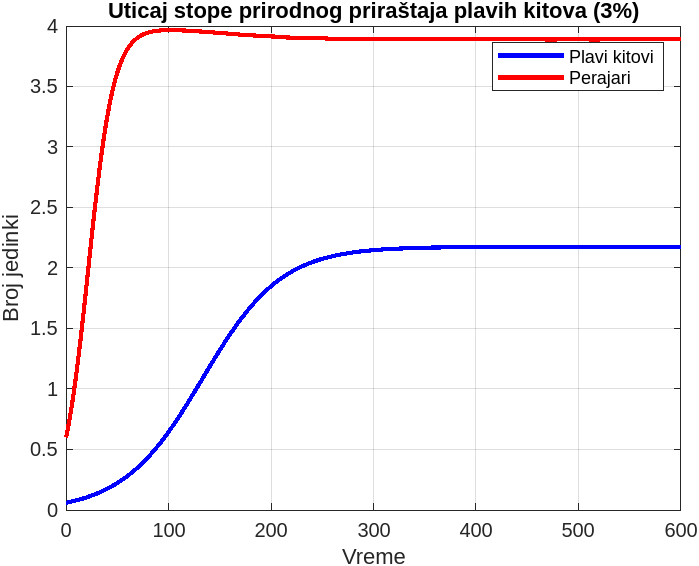
\includegraphics[width=\textwidth]{uticaj3.png}
			\caption{Priraštaj za 3\%}
			\label{slika1: uticaj3}
		\end{minipage}
		\hspace{0.5cm} 
		\begin{minipage}[h]{0.45\linewidth}
			\centering
			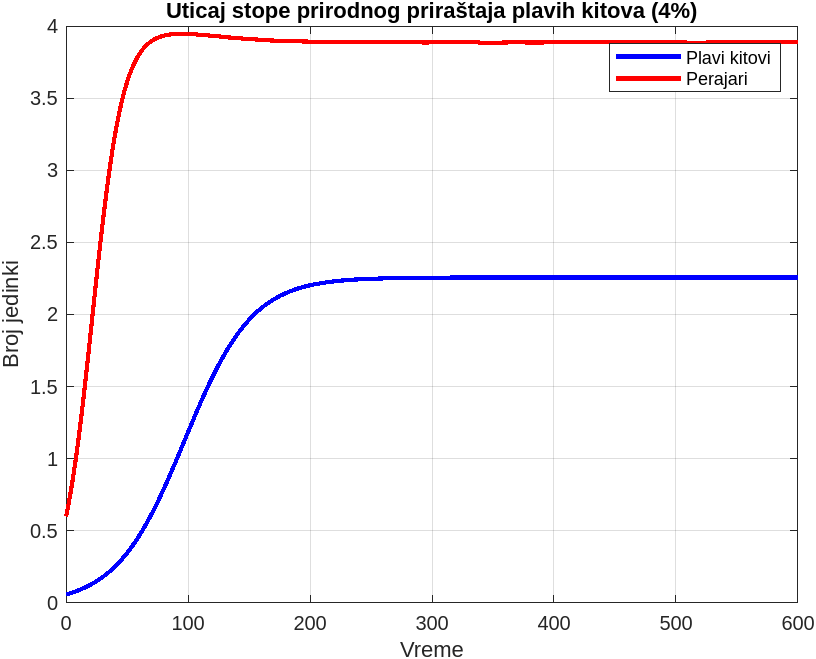
\includegraphics[width=\textwidth]{uticaj4.png} 
			\caption{Priraštaj za 4\%} 
			\label{slika2: uticaj4}
		\end{minipage}
	\end{figure}

	Kod stope prirodnog priraštaja od 3\% (Slika 4) i 4\% (Slika 5), primećujemo da je rast populacije brži u odnosu na 2\%. Populacija će dostići stabilnu tačku, koja je nešto viša u odnosu sa nižom stopom prirodnog priraštaja. Time konkurencija sa kitovima perajarima postaje značajnija, ali će i dalje biti kontrolisana. Populacija plavih kitova raste umereno i stabilizuje se na višem nivou. Konkurencija za resurse je intezivnija, ali ne dovodi do izumiranja.
	
	\newpage
	
	\subsection{Visoka stopa priraštaja (6-7\%)}
	
	\begin{figure}[h]
		\centering
		\begin{minipage}[h]{0.45\linewidth}
			\centering
			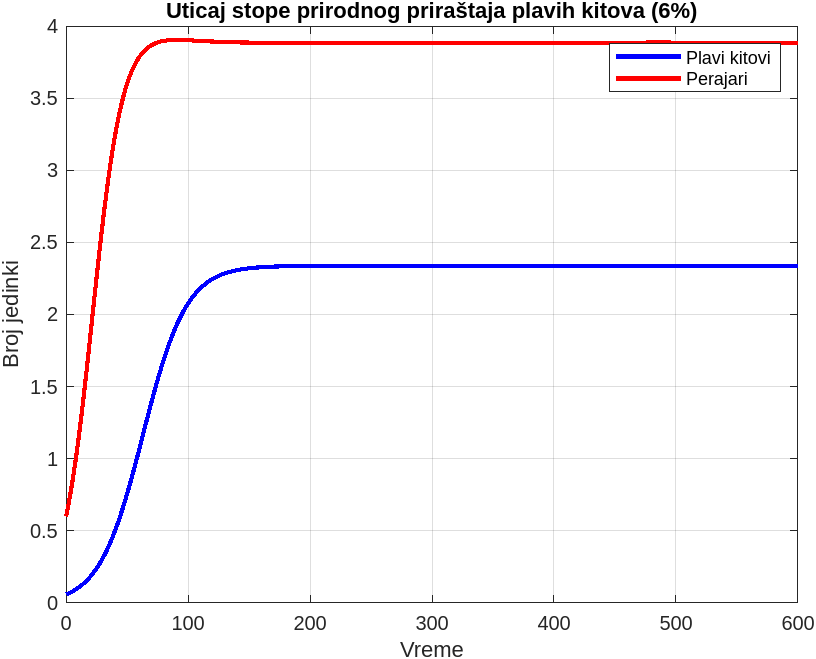
\includegraphics[width=\textwidth]{uticaj6.png}
			\caption{Priraštaj za 6\%}
			\label{slika1: uticaj6}
		\end{minipage}
		\hspace{0.5cm} 
		\begin{minipage}[h]{0.45\linewidth}
			\centering
			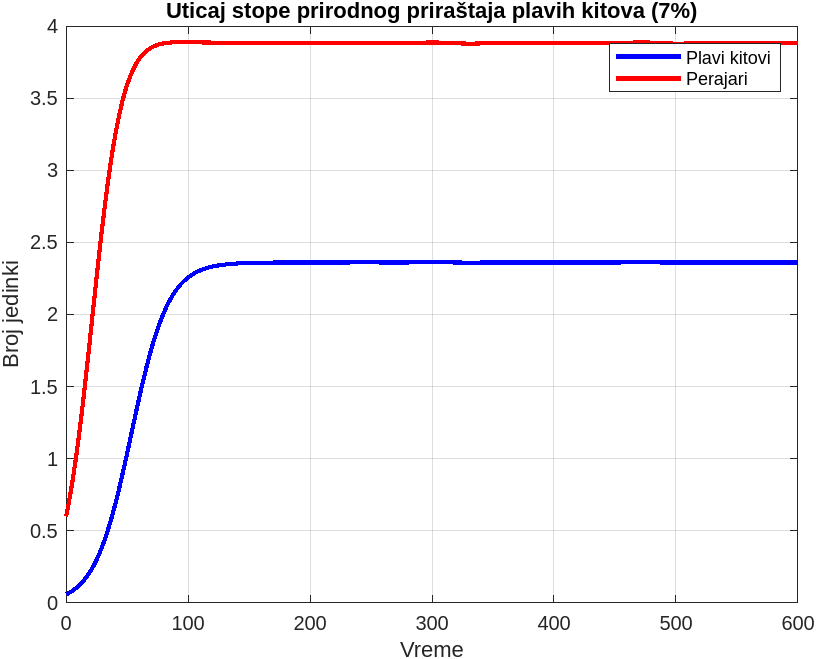
\includegraphics[width=\textwidth]{uticaj7.png} 
			\caption{Priraštaj za 7\%} 
			\label{slika2: uticaj7}
		\end{minipage}
	\end{figure}

	\iffalse
	Stope prirodnog priraštaja od 6\% i 7\% dovode do bržeg rasta plavih kitova. Kako mogu brzo dostići kapacitet svog prirodnog staništa, to može dovesti to veće konkurencije sa kitovima perajarima. To dalje može da dovede do nestabilnosti pre nego što se postignu stabilne ravnotežne tačke. 
	\fi
	
	Stope prirodnog priraštaja od 6\% (Slika 6) i 7\% (Slika 7) značajno utiču na dinamiku populacija plavih kitova, a tako i na kitove perajare. Sa ovim stopama prirodnog priraštaja, populacija plavih kitova raste veoma brzo i to dovodi do bržeg dostizanja kapaciteta staništa. Ovo povećava konkurenciju između dve vrste za resurse i to može da izazove oscilacije u populaciji i moguću nestabilnost pre nego što se dostigne stabilna tačka. 
	\iffalse 
	Ovakve oscilacije predstavljaju periodične promene u broju jedinki pre nego što se populacije stabilizuju svoje brojčano stanje. 
	\fi 
	
	\subsection{Opšti zaključak}
	\label{sec: opsti-zakljucak}
	
	\begin{figure}[h]
		\centering
		\begin{minipage}[h]{0.45\linewidth}
			\centering
			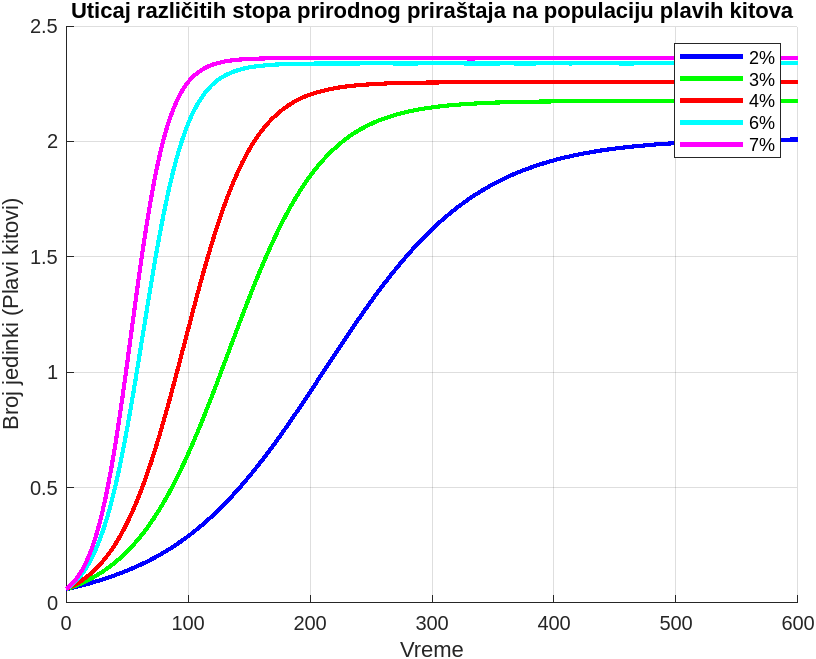
\includegraphics[width=\textwidth]{plaviQ.png}
			\caption{Grafik stopa prirodnih priraštaja za plave kitove}
			\label{slika1: uticaj6}
		\end{minipage}
		\hspace{0.5cm} 
		\begin{minipage}[h]{0.45\linewidth}
			\centering
			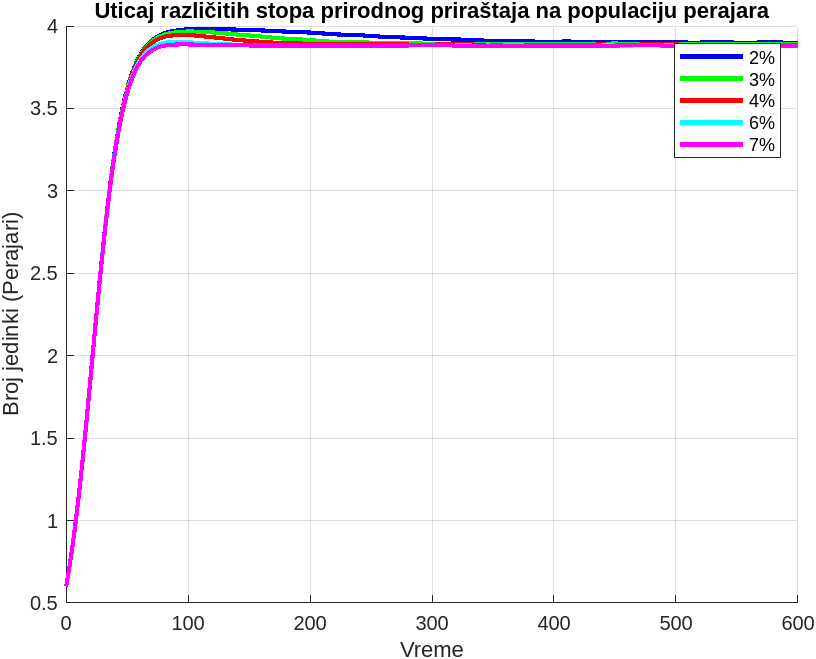
\includegraphics[width=\textwidth]{perajariQ.png} 
			\caption{Grafik stopa prirodnih priraštaja za kitove perajare} 
			\label{slika2: uticaj7}
		\end{minipage}
	\end{figure}
	
	Zaključujemo da povećanjem parametra prirodnog priraštaja populacija raste brže nego pre, odnosno plavi kitovi će za kraće vreme dostići stabilnu tačku. Ako je stopa prirodnog priraštaja plavih kitova niska, populacija plavih kitova će rasti sporije (Slika 8). Ovo omogućava populaciji kitova perajara da se stabilizuju na vecoj tački (Slika 9). Povećanjem stope prirodnog priraštaja plavih kitova vodi ka većoj populaciji i povećanjem stacionarnih tačaka, što povećava konkurenciju za resurse i dovodi do smanjenja stacionarnih tačaka populacije perajara. 
	
	\iffalse
	Povećanjem stope prirodnog priraštaja plavih kitova (Slika 8), dolazi do bržeg rasta njihove populacije. To vodi ka intezivnijoj konkurenciji za resurse, što utiče na smanjenje stacionarne tačke populacije kitova perajara (Slika 9). 
	 
	Kada je stopa priraštaja plavih kitova visoka, to dovodi do povećanja njihove populacije i samim tim se povećava konkurencija za resurse, što dovodi do smanjena stacionarnih tačaka populacije kitova perajara. 
	\fi
	
	\newpage
	
	\section{Lov na kitove}
	\label{sec: lov-na-kitove}
	
	Kako bismo obuhvatili ribolov, možemo proširiti model dodavanjem novih parametara diferencijalnim jednačinama koje opisuju ulov kitova od strane brodova koji ih love. Ovaj uslov možemo opisati sa stopom ulova \textit{q}, koja predstavlja procenat populacije koja se godišnje ulovi brodovima. Evo kako možemo izmeniti početne diferencijalne jednačine, tako da one sad predstavljaju zadati opisani problem:\\ 
	\\

	\[
		\frac{dx}{dt} = 0.05x(1 - \frac{x}{250000}) - axy - Eqx
	\]
	\[
		\frac{dy}{dt} = 0.08y(1 - \frac{y}{400000}) - axy - Eqy
	\]
	\\

	Parametar E predstavlja koliko brodova učestvuje u lovu na kitove.\\
	\\
	Kako bismo odredili maksimalan broj brodova $E$ koji mogu loviti kitove, a da pritom ne dođe do izumiranja bilo koje vrste potrebno je da nađemo ravnotežne tačke ovog sistema.\\ 
	\\
	To radimo tako što početne jednačine izjednačimo sa nulom i rešimo sistem:
	
	\setcounter{equation}{0}
	\begin{equation}
		0.05x(1 - \frac{x}{250000}) - axy - qEx = 0
	\end{equation}
	
	
	\begin{equation}
		0.08y(1 - \frac{y}{400000}) - axy - qEy = 0
	\end{equation}
	
	Iz jednačine (1) možemo da izvučemo $x$, a iz jednačine (2) možemo da izvučemo $y$, i dobijamo sledeće:\\
	
	\begin{equation}
		x \cdot (0.05(1 - \frac{x}{250000}) - ay - qE) = 0
	\end{equation}

	\begin{equation}
		y \cdot (0.08(1 - \frac{y}{400000}) - ax - qE) = 0
	\end{equation}
	
	Iz jednačine (3) dobijamo da je $x = 0$ ili da je sledeći izraz jednak nuli:
	
	\[
		0.05(1 - \frac{x}{250000}) - ay - qE = 0
	\]
	
	Sređujemo ovaj izraz po $x$ i dobijamo:
	
	\[
		x = 25 \cdot 10^{4} - 5\cdot 10^{6}(ay + qE)
	\]
	Odnosno, kada zamenimo poznate parametre $a = 10^{-8}$ i $q = 10^{-5}$ dobijamo:
	
	\begin{equation}
		x = 25 \cdot 10^{4} - 5 \cdot 10^{-2} y - 50E
	\end{equation}

	Iz jednačine (4) dobijamo da je $y = 0$ i sledeći izraz da je jednak nuli:
	
	\[
		0.08(1 - \frac{y}{400000}) - ax - qE = 0
	\]
	
	Sređujemo izraz po $y$, i dobijamo sledeći izraz:
	
	\[
		y = 4 \cdot 10^{5} - 5 \cdot 10^{6} ax - 5 \cdot 10^{6} qE
	\]
	
	Odnosno kada ubacimo konkretne vrednosti za parametre $a = 10^{-8}$ i $q = 10^{-5}$, dobijamo:
	
	\begin{equation}
		y = 4 \cdot 10^{5} - 5 \cdot 10^{-2} x - 50E
	\end{equation}

	%Kako bismo osigurali da obe vrste kitova dostignu svoje pozitivne %ravnotežne tačke treba isputnit da su $x > 0$ i $y > 0$. 
	Ravnotežne tačke zavise od broja brodova $E$. Da bi se održala stabilna populacija obe vrste kitova, $x$ i $y$ moraju biti pozitivni.Prenesemo to sad na jednačine (5) i (6):
	
	\[
		25 \cdot 10^{4} - 5 \cdot 10^{-2} y - 50E > 0
	\]	  
	
	\[
		4 \cdot 10^{5} - 5 \cdot 10^{-2} x - 50E > 0
	\]
	
	Ove nejednačine izrazimo tako da samo sa jedne strane imamo čisto $E$, posle njihovog sređivanja dobijamo:
	
	\begin{equation}
		E < 5000 - 0.001y
	\end{equation}

	\begin{equation}
		E < 8000 - 0.001x
	\end{equation}
	
	Nejednačine (7) i (8) možemo jedinstevno zapisati kao sledeći izraz:
	
	\begin{equation}
		E < min(5000 - 0.001y, 8000 - 0.001x)
	\end{equation}

	Ovako dobijeni izraz nam određuje maksimalan broj brodova $E$. Ovo ograničenje nam osigurava da populacije ostanu pozitivne i stabilne. Najveći broj kitova koji može biti ulovljen, a da pritom ne dođe do izumiranja bilo koje vrste, zavisi od kombnacije ovih parametara. Kako bismo precizno odredili opseg, potrebno je ubaciti početne uslove, a to su $x(0) = 6000$ i $y(0) = 60000$.
	
	\begin{equation}
		E < min(4940, 7994)
	\end{equation}

	Kako je opseg minimum ovde dve vrednosti sledi da je 
	
	\begin{equation}
		E < 4940
	\end{equation}
		
	
	Maksimalan broj brodova $E$ koji može uloviti kitove, a da pritom ne dođe do izumiranja bilo koje vrste je $4940$. Ovo osigurava da se populacije stabilizuju na pozitivnim ravnotežnim tačkama. Stoga zaključujemo da broj brodova mora biti manji od 4940 kako bi izbegli izumiranje kitova.
	
	
	%Najveći broj brodova $E$koji može loviti kitove bez dovođenja do izumiranja bilo koje vrste je $E = ...$ i  time se osigurava stabilnost populacije. 
	
	\iffalse
	Za određivanje opsega za broj brodova E za koje će se broj kitova obe vrste približiti pozitivnoj ravnotežnoj tački, možemo koristiti numeričke metode za rešavanje sistema diferencijalnih jednačina za različite vrednosti parametra E. Kada se broj kitova približava pozitivnoj ravnotežnoj tački, to znači da uslov nije dovoljan da značajnije utiče na brojnost populacije. \\
	
	\newpage
	
	\subsection{Analiza grafika sa stopom ulova}
	\label{sec: analiza-grafika-sa-stopm-ulova}
	
	Naredni grafik prikazuje za parametre lova a = $10^{-8}$ i stopu ulova q = $10^{-5}$ i broj brodova koji učestvuje u lovu E = 28000000.
	
	\begin{figure}[h]
		\centering
		\begin{minipage}[h]{0.45\linewidth}
			\centering
			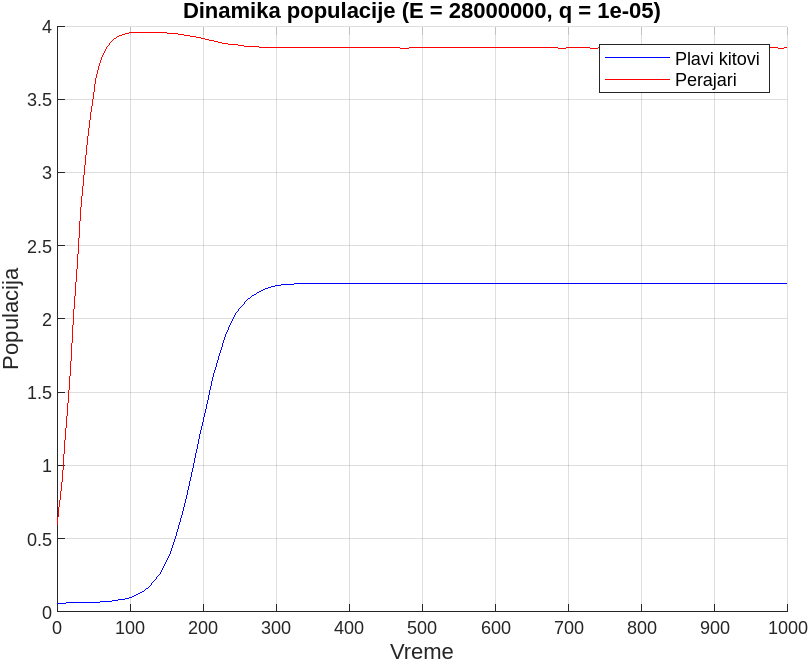
\includegraphics[width=\textwidth]{lov1.png}
			\caption{Lov na kitove: \\E = $28000000$ i q = $10^{-5}$}
			\label{slika1: lov-1}
		\end{minipage}
	\end{figure}
	
	
	Na početku, možemo da primetimo da obe vrste kitova rastu. To je zbog toga što su početne populacije male u odnosu sa kapacitetom njigovih staništa. Broj kitova perajara nam se povećava od početne vrednosti od 60000 jedinki, dok se plavi kitovi povećavaju od početne vrednosti 6000 jedinki. \\
	\\
	Vidimo da se nakon 300 vremenskih jednica, populacija plavih kitova, a to nam je plava kriva na grafikonu dostiže stabilnu tačku na populaciji oko 2.2 jedniki. Dok, kitovi perajari nakon 100 vremenskih jedinica dostižu stabilnu tačku na populaciji oko 3.8 jedinki. \\ 
	\\
	Primećujemo da lov ima veliki uticaj na obe populacije. Parametar \textit{qE} koji predstavlja ukupnu stopu ulova utiče na brzinu smanjenja populacija nakon što one dostignu svoje stabilne tačke. U ovako zabeleženom scenariju, stopa ulova je dovoljno visoka da spreči da populacije dalje rastu do njihovog maksimalnog potencijala. To nije dovoljno visoka vrednost da bi dovela do izumiranja bilo koje vrste kitova. \\ 
	\\ 
	U ovoj simulaciji, postignut je balans gde nijedna vrsta nije izumrla, dok su njihove populacije održane na stabilnom nižem nivou, nego što bi bile u odsustvu lova. \\
	\\
	\newpage
	Sada prelazimo na analizu narednog grafika, sa sledećim parametrima: a = $10^{-8}$, q = $10^{-5}$, E = $28198666.7$.
	
	\begin{figure}[h]
		\centering
		\begin{minipage}[h]{0.45\linewidth}
			\centering
			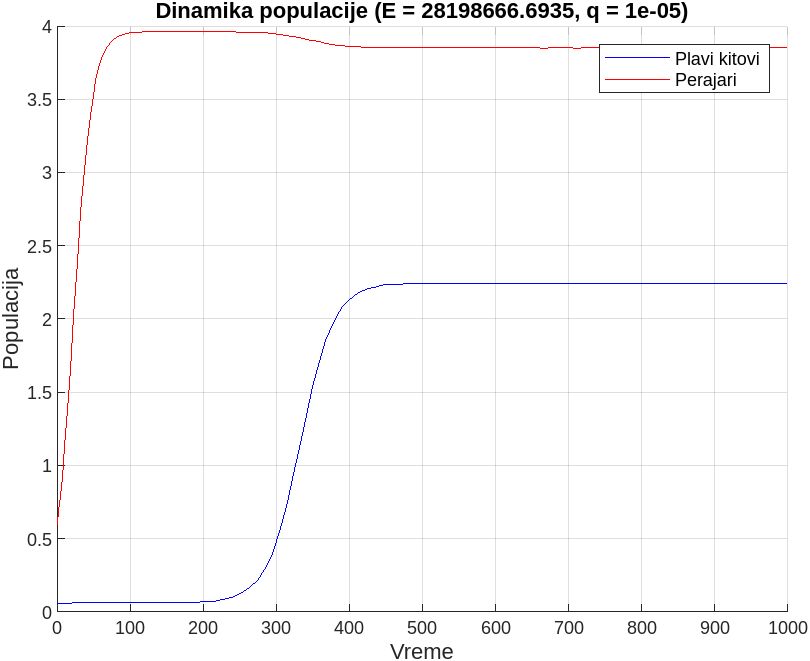
\includegraphics[width=\textwidth]{lov2.png}
			\caption{Lov na kitove: \\E = $2819866$ i q = $10^{-5}$}
			\label{slika1: lov-2}
		\end{minipage}
	\end{figure}
	
	
	Primećujemo da se u periodu do 100 vremenskih jedinica, broj jedinki kod obe vrste raste. Populacija kitova perajara dosta brže raste u odnosu na plave kitove, a to je zbog toga što ih ima deset puta više. \\
	Nakon, 100 vremenskih jedinica, vidimo da populacija kitova perajara dostiže dostiže stabilnu tačku. Dok, populaciju plavih kitova nastavlja da raste sve do 400 vremenskih jedinica. \\
	\\
	Primećujemo da su različiti obrasci rasta i stabilizacije plavih kitova i kitova perajara. Perajari dostižu svoju ravnotežnu tačku i na višem nivou u poređenju sa plavim kitovima.\\
	\\
	Dolazimo do zaključka da je maksimalni dozvoljeni broj brodova koji može da lovi 28199126, time se ostvaruje maksimalni ulov od 282 jedinke čime ne dovodi do istrebljenja bilo koje vrste.
	\fi
	
	\newpage
	
	\section{Zaključak}
	\label{sec: zakljucak}
	
	U ovom radu smo analizirali matematički model interakcije dve vrste kitova - plavih kitova i kitova perajara, koji se takmiče za hranu, koristeći sistem diferencijalnih jednačina. Cilj je bio razumeti kako različiti faktori kao što su prirodni priraštaj, konkurencija za resurse i ribolov mogu uticati na dinamiku ovih populacija. \\
	\\
	Glavni zaključci su sledeći: \\ 
	
	\begin{enumerate}
		
		\item \textbf{Stacionarna rešenja}: Analizom stacionarnih rešenja otkriveno je nekoliko ravnotežnih tačaka. Na primer, tačke $(250000, 0)$ i $(0, 400000)$ nam predstavljaju situcaije u kojima jedna vrsta izumire dok druga dostiže stabilnost. Ove tačke su nestabilne, a to znači da su osetljive na male promene u početnim uslovima, a to dalje ukazuje na potencijalnu nestabilnost u ekosistemu.
		
		\item \textbf{Konkurencija za resurse}: Konkurencija između dve vrste kitova može dovesti do izumiranja jedne vrste ukoliko je ta konkurencija previše intezivna. Kada je parametar konkurencije manji, odnosno $a = 10^{-8}$, tada je ta konkurencija manje izražena i populacije imaju tendenciju da dostignu svoje stabilne tačke. Nasuprot tome, kada je $a$ veći, odnosno $a = 10^{-6}$, konkurencija je intezivnija i to dovodi do izumiranja plavih kitova. Ove različite vrednosti nam pružaju uvid u tome kako interakcija između vrsta utiče na stabilnost njihovih populacija. 
		
		\item \textbf{Promena prirodnog priraštaja}: Razmatranjem različitih stopa prirodnog priraštaja kod plavih kitova, ustanovljeno je da će veće stope priraštaja omogućavati brži oporavak populacije, ali i dalje zavise od inteziteta konkurencije sa kitovima perajarima. U većini slučajeva, veći prirodni priraštaj doprinosi stabilnosti populacije plavih kitova, ali ne može u ptpunosti neutralisati negativne efekte konkurencije. 
		
		\item \textbf{Uticaj ribolova}: Uvođenjem robilova u model, analizirali smo kako različite stope ulova i  broj brodova utiču na populaciju kitova. Zaključili smo da postoji određeni opseg broja brodova $E$ i stope ulova $q$ za koje populacije obe vrste mogu dostići stabilne tačke bez rizika da će izumreti. Prekoračenje ovog opsega može dovesti ozbiljih ekoloških posledica, uključujući i izumiranje jedne ili pak obe populacije. 
		
		
	\end{enumerate}
	
	
	
	%Naša analiza pokazuje da parametri kao što su stopa prirodnog priraštaja i ribolova imaju značajan uticaj na dinamiku populacija kitova. Pravilno postavljanje i kontrola ovih parametara mogu pomoći u očuvanju populacija obe vrste kitova. Modeli i simulacije koje smo razvili pružaju vredne alate za bolje razumevanje i upravljanje ovim važnim ekosistemima.
	
	
	
		
	\newpage	
		
	\addcontentsline{toc}{section}{Literatura}
	\appendix
		
	\begin{thebibliography}{9}
		\bibitem{knjiga} Milan Dražić, \textit{Matematičko modeliranje}, Univerzitet u Beogradu Matematički fakultet, 2017.
		
		\bibitem{jedna-vrsta} Zorica Dražić, Populacioni model jedne vrste: \url{https://poincare.matf.bg.ac.rs/~zorica.drazic/OMM/04 - OMM - populacioni_a.pdf}
		
		\bibitem{vise-vrsta} Zorica Dražić, Populacioni modeli više vrsta \url{https://poincare.matf.bg.ac.rs/~zorica.drazic/OMM/04%20-%20OMM%20-%20populacioni.pdf}
						
	\end{thebibliography}
		
		
		
		
		
		
		
		
		
		
		
		
		
		
		
		
		
		
		
		
		
		
		
		
		
		
		
		
	\end{document}